%--------1---------2---------3---------4---------5---------6---------7---------8
\documentclass[11pt,a4paper]{article}%
% //////////////////////////////////////////////////////////////////////////////
\title{Fluid Mechanics 2\\Problem Sets \\2020/21}
%\author[]{Imperial College London \\ Mechanical Engineering Department}%
\date{}
% //////////////////////////////////////////////////////////////////////////////

\usepackage[a4paper,top=2cm,bottom=2cm,left=2cm,right=2cm]{geometry}%
\usepackage{lmodern}%                     font style must be sans serif to
\renewcommand*\familydefault{\sfdefault}% comply with the college's regulations
\usepackage[T1]{fontenc}%                 with respect to disabilities!
\usepackage{pifont}
\usepackage{fancyhdr}
    \pagestyle{fancy}
    \fancyhf{}
    \renewcommand{\headrulewidth}{0pt}
    \lfoot{\ifnum0<\thesection Set \# \leftmark\fi}
    \rfoot{\thepage}
 
%\usepackage[cmbright]{sfmath}           % This part for the math font, but it causes a lot of errors
%\usepackage{helvet}%
% ------------------------------------------------------------------------------
\usepackage{lipsum}% for dummy text
\usepackage{booktabs}% for nicely typeset tabular material
\usepackage[hidelinks]{hyperref}%
\usepackage{graphicx}% for graphics
\setkeys{Gin}{width=\linewidth,totalheight=\textheight,keepaspectratio}
\graphicspath{{figs/}}
%
% The fancyvrb package lets us customize the formatting of verbatim
% environments.  We use a slightly smaller font.
\usepackage{fancyvrb}
\fvset{fontsize=\normalsize}
\usepackage{xspace}% prints a trailing space in a smart way.
\usepackage{units}%
\usepackage{makeidx}%
\usepackage{tcolorbox}%
\tcbuselibrary{breakable}%
\tcbuselibrary{skins}%
%\tcbset{mytitle/.style={title={Task~\thetcbcounter\ifstrempty{#1}{}{\thechapter.#1:#1}}}}
\newtcolorbox{cbox}{colback=red!2!white,colframe=red!50!white,arc=10pt,boxrule=.5pt,skin=enhanced,breakable}
\newtcolorbox[auto counter, number within=chapter, number freestyle={\noexpand\thechapter.\noexpand\arabic{\tcbcounter}}]{cboxt}[2][]{%
    colback=red!2!white,
    colframe=red!50!white,
    enhanced,
    breakable,
    arc=10pt,boxrule=.5pt,
    fonttitle=\bfseries,
    title=Task~\thetcbcounter: #2,
    #1
}
\newtcolorbox{exobox}[1]{colback=black!1!white,colframe=black!60!white,fonttitle=\bfseries,title=#1,arc=5pt,boxrule=.5pt,skin=enhanced,breakable}
\newtcolorbox{readlist}{colback=blue!2!white,colframe=blue!50!white,arc=10pt,boxrule=.5pt,skin=enhanced,breakable}
\definecolor{kecolour}{rgb}{0,0.5,0}
\newtcolorbox{keyeqn}[1]{colback=kecolour!1!white,colframe=kecolour,fonttitle=\bfseries,title=#1,arc=3pt,boxrule=.5pt,skin=enhanced,breakable}
\definecolor{wkdcolour}{rgb}{0,0.4,0.9}
\newtcolorbox{wkdex}[1]{colback=wkdcolour!1!white,colframe=wkdcolour,fonttitle=\bfseries,title=#1,arc=3pt,boxrule=.5pt,skin=enhanced,breakable}

%
\usepackage{enumerate}%
%
\usepackage{amsmath,mathtools}%
% Boxes around equations
\usepackage{empheq}\newcommand*\widefbox[1]{\fbox{\hspace{2em}#1\hspace{2em}}}
\usepackage{amssymb}%
\usepackage{amsfonts}%
%\usepackage{accents}%
\usepackage{bm}%
\usepackage{upgreek}%
\usepackage{stmaryrd}%
\usepackage{mathrsfs}%
\usepackage{tikz}%
    \newcommand*\circled[1]{\tikz[baseline=(char.base)]{
            \node[shape=circle,draw,inner sep=2pt] (char) {#1};}}
%
\usepackage{longtable}%
\usepackage{tabularx}
%
\usepackage{wasysym}%
\usepackage{pdfpages}%
\usepackage{csquotes}% For quotes (use \begin{displayquote})
\usepackage{cancel} % To cancel out terms in an equation
\usepackage{float}      % To place tables with text using [H]
\restylefloat{table}    % To place tables with text using [H]
\usepackage{nameref}    % To refer to lecture names
\usepackage{xcolor}     % Coloured text



% Bibliography
\usepackage{natbib}
 
 
 
%
% ------------------------------------------------------------------------------
% Images before chapters
\newcommand\ChapImage{}
% Prints argument within hanging parentheses (i.e., parentheses that take
% up no horizontal space).  Useful in tabular environments.
\newcommand{\hangp}[1]{\makebox[0pt][r]{(}#1\makebox[0pt][l]{)}}
%
% Prints an asterisk that takes up no horizontal space.
% Useful in tabular environments.
\newcommand{\hangstar}{\makebox[0pt][l]{*}}
%
% Some shortcuts for Tufte's book titles.  The lowercase commands will
% produce the initials of the book title in italics.  The all-caps commands
% will print out the full title of the book in italics.
\newcommand{\vdqi}{\textit{VDQI}\xspace}
\newcommand{\ei}{\textit{EI}\xspace}
\newcommand{\ve}{\textit{VE}\xspace}
\newcommand{\be}{\textit{BE}\xspace}
\newcommand{\VDQI}{\textit{The Visual Display of Quantitative Information}\xspace}
\newcommand{\EI}{\textit{Envisioning Information}\xspace}
\newcommand{\VE}{\textit{Visual Explanations}\xspace}
\newcommand{\BE}{\textit{Beautiful Evidence}\xspace}
%
\newcommand{\TL}{Tufte-\LaTeX\xspace}
%
% Prints the month name (e.g., January) and the year (e.g., 2008)
\newcommand{\monthyear}{%
  \ifcase\month\or January\or February\or March\or April\or May\or June\or
  July\or August\or September\or October\or November\or
  December\fi\space\number\year
}%
% Prints an epigraph and speaker in sans serif, all-caps type.
\newcommand{\openepigraph}[2]{%
  %\sffamily\fontsize{14}{16}\selectfont
  \begin{fullwidth}
  \sffamily\large
  \begin{doublespace}
  \noindent\allcaps{#1}\\% epigraph
  \noindent\allcaps{#2}% author
  \end{doublespace}
  \end{fullwidth}
}%
% Inserts a blank page
\newcommand{\blankpage}{\newpage\hbox{}\thispagestyle{empty}\newpage}
%
% Typesets the font size, leading, and measure in the form of 10/12x26 pc.
\newcommand{\measure}[3]{#1/#2$\times$\unit[#3]{pc}}%
% Macros for typesetting the documentation
\newcommand{\hlred}[1]{\textcolor{Maroon}{#1}}% prints in red
\newcommand{\hangleft}[1]{\makebox[0pt][r]{#1}}
\newcommand{\hairsp}{\hspace{1pt}}% hair space
\newcommand{\hquad}{\hskip0.5em\relax}% half quad space
\newcommand{\TODO}{\textcolor{red}{\bf TODO!}\xspace}
\newcommand{\ie}{\textit{i.\hairsp{}e.}\xspace}
\newcommand{\eg}{\textit{e.\hairsp{}g.}\xspace}
\newcommand{\na}{\quad--}% used in tables for N/A cells
\providecommand{\XeLaTeX}{X\lower.5ex\hbox{\kern-0.15em\reflectbox{E}}\kern-0.1em\LaTeX}
\newcommand{\tXeLaTeX}{\XeLaTeX\index{XeLaTeX@\protect\XeLaTeX}}
% \index{\texttt{\textbackslash xyz}@\hangleft{\texttt{\textbackslash}}\texttt{xyz}}
\newcommand{\tuftebs}{\symbol{'134}}% a backslash in tt type in OT1/T1
\newcommand{\doccmdnoindex}[2][]{\texttt{\tuftebs#2}}% command name -- adds backslash automatically (and doesn't add cmd to the index)
\newcommand{\doccmddef}[2][]{%
  \hlred{\texttt{\tuftebs#2}}\label{cmd:#2}%
  \ifthenelse{\isempty{#1}}%
    {% add the command to the index
      \index{#2 command@\protect\hangleft{\texttt{\tuftebs}}\texttt{#2}}% command name
    }%
    {% add the command and package to the index
      \index{#2 command@\protect\hangleft{\texttt{\tuftebs}}\texttt{#2} (\texttt{#1} package)}% command name
      \index{#1 package@\texttt{#1} package}\index{packages!#1@\texttt{#1}}% package name
    }%
}% command name -- adds backslash automatically
\newcommand{\doccmd}[2][]{%
  \texttt{\tuftebs#2}%
  \ifthenelse{\isempty{#1}}%
    {% add the command to the index
      \index{#2 command@\protect\hangleft{\texttt{\tuftebs}}\texttt{#2}}% command name
    }%
    {% add the command and package to the index
      \index{#2 command@\protect\hangleft{\texttt{\tuftebs}}\texttt{#2} (\texttt{#1} package)}% command name
      \index{#1 package@\texttt{#1} package}\index{packages!#1@\texttt{#1}}% package name
    }%
}% command name -- adds backslash automatically
\newcommand{\docopt}[1]{\ensuremath{\langle}\textrm{\textit{#1}}\ensuremath{\rangle}}% optional command argument
\newcommand{\docarg}[1]{\textrm{\textit{#1}}}% (required) command argument
\newenvironment{docspec}{\begin{quotation}\ttfamily\parskip0pt\parindent0pt\ignorespaces}{\end{quotation}}% command specification environment
\newcommand{\docenv}[1]{\texttt{#1}\index{#1 environment@\texttt{#1} environment}\index{environments!#1@\texttt{#1}}}% environment name
\newcommand{\docenvdef}[1]{\hlred{\texttt{#1}}\label{env:#1}\index{#1 environment@\texttt{#1} environment}\index{environments!#1@\texttt{#1}}}% environment name
\newcommand{\docpkg}[1]{\texttt{#1}\index{#1 package@\texttt{#1} package}\index{packages!#1@\texttt{#1}}}% package name
\newcommand{\doccls}[1]{\texttt{#1}}% document class name
\newcommand{\docclsopt}[1]{\texttt{#1}\index{#1 class option@\texttt{#1} class option}\index{class options!#1@\texttt{#1}}}% document class option name
\newcommand{\docclsoptdef}[1]{\hlred{\texttt{#1}}\label{clsopt:#1}\index{#1 class option@\texttt{#1} class option}\index{class options!#1@\texttt{#1}}}% document class option name defined
\newcommand{\docmsg}[2]{\bigskip\begin{fullwidth}\noindent\ttfamily#1\end{fullwidth}\medskip\par\noindent#2}
\newcommand{\docfilehook}[2]{\texttt{#1}\index{file hooks!#2}\index{#1@\texttt{#1}}}
\newcommand{\doccounter}[1]{\texttt{#1}\index{#1 counter@\texttt{#1} counter}}
\usepackage{wrapfig}%
%-------------------------------------------------------------------------------
% Section titles
\newcommand{\secname}{CIVE40008-hFMX Problem Set \#}
\usepackage{titlesec}
\titleformat{\section}
{\normalfont\bfseries\filcenter\large}
{CIVE40008 Problem Set \#\thesection ~---}{0.5 em}{}



% Pasted form the lecture notes but will need updating as hard coded:
\newcommand{\fig}[1]{Fig.~\ref{fig:#1}}%
\renewcommand{\figurename}{Fig.}%
\newcommand{\eqn}[1]{Eq.~\ref{eqn:#1}}%
\newcommand{\eqns}[2]{Eqs.~\ref{eqn:#1}--\ref{eqn:#2}}%
\newcommand{\etal}{ et al.}%
%-------------------------------------------------------------------------------
% OPERATORS
%\renewcommand{\vec}[1]{\underaccent{\bar}{#1}}% vectors
\newcommand{\vect}[1]{\bm{#1}}% vectors
\newcommand{\matl}[1]{\underline{\underline{#1}}}% tensors
\newcommand{\mat}[1]{\mathbf{#1}}% tensors

\newcommand{\grad}[1]{\mathbf{grad}(#1)} % grad of a scalar (bold)
\newcommand{\grada}[1]{\overrightarrow{\textrm{grad}}(#1)} % grad of a scalar (arrow)
\newcommand{\gradva}[1]{\matl{\textrm{grad}}(\Vec{#1})} % grad of a vector (arrow)
\newcommand{\ngrad}[1]{\vect{\nabla}#1} % grad of a scalar (bold)
\newcommand{\ngrada}[1]{\Vec{\nabla}#1} % grad of a scalar (arrow)
\newcommand{\gradv}[1]{\mathbf{grad}(\vect{#1})} % grad of a vector
\newcommand{\ngradv}[1]{\vect{\nabla}\vect{#1}} % grad of a vector
\newcommand{\divv}[1]{\mathrm{div}(\vect{#1})}% div of a vector (bold)
\newcommand{\divva}[1]{\mathrm{div}(\Vec{#1})}% div of a vector (arrow)
\newcommand{\ndivv}[1]{\nabla\cdot\vect{#1}}% div of a vector
\newcommand{\divp}[1]{\mathrm{div}(#1)}% div of a product
\newcommand{\ndivp}[1]{\nabla\cdot(#1)}% div of a product
\newcommand{\divt}[1]{\mathbf{div}(\mat{#1})}% div of a tensor
\newcommand{\ndivt}[1]{\vect{\nabla}\cdot\mat{#1}}% div of a tensor
\newcommand{\divta}[1]{\overrightarrow{\mathrm{div}}(\matl{#1})}% div of a tensor (arrow)
\newcommand{\divtp}[1]{\mathbf{div}(#1)}% div of a tensor product
\newcommand{\ndivtp}[1]{\vect{\nabla}\cdot (#1)}% div of a tensor product
\newcommand{\curl}[1]{\mathbf{rot}(\mat{#1})}% curl of a vector (bold)
\newcommand{\ncurl}[1]{\vect{\nabla}\times\vect{#1}}% curl (nabla x) of a vector
\newcommand{\curlva}[1]{\overrightarrow{\mathrm{curl}}(\Vec{#1})}% curl of a vector (arrow)
\newcommand{\DD}{\textrm{D}} % Big D operator
\newcommand{\dd}{\textrm{d}} % Normal d operator
\newcommand{\pd}{\partial} % Partial d operator

\newcommand{\tr}{^{\mathrm{t}}}% transpose

% NON-DIM NUMBERS
\newcommand{\Kn}{\mathrm{Kn}}%
\newcommand{\Ma}{\mathrm{M}}%
\newcommand{\Pra}{\mathrm{Pr}}%
\newcommand{\Rey}{\mathrm{Re}}%

% MISC
\newcommand{\vmol}{\vect{u}_p}% molecular velocity vector

\newcommand{\rbar}{\skew3\bar{\rho}}%
\newcommand{\ubar}{\skew2\bar{u}}%
\newcommand{\pbar}{\skew3\bar{p}}%
\newcommand{\mbar}{\skew3\bar{\vect{\mu}}}%
\newcommand{\Abar}{\skew0\bar{\mat{A}}}%
\newcommand{\Nbar}{\skew0\bar{\mat{N}}}%
\newcommand{\Jbar}{\skew2\bar{\mat{J}}}%
\newcommand{\Kbar}{\skew0\bar{\mat{K}}}%
\newcommand{\cbar}{\skew3\bar{c}}%
\newcommand{\qbar}{\skew3\bar{\vect{q}}}%
\newcommand{\usbar}{\skew2\bar{u}_s}%
\newcommand{\etbar}{\skew3\bar{e}_t}%
\newcommand{\varthetabar}{\skew3\bar{\vartheta}}%

\newcommand{\rp}{\rho^\prime}%
\newcommand{\up}{u^\prime}%
\newcommand{\pp}{p^\prime}%
\newcommand{\mup}{\vect{\mu}^\prime}%
\newcommand{\qp}{\vect{q}^\prime}%
\newcommand{\usp}{u_s^\prime}%

% Stress tensor
\newcommand{\sigii}{
        \begin{bmatrix}
            \sigma_{11} & \sigma_{12} & \sigma_{13} \\
            \sigma_{21} & \sigma_{22} & \sigma_{23} \\
            \sigma_{31} & \sigma_{32} & \sigma_{33}
        \end{bmatrix}}

\newcommand{\ETrule}{
\begin{center}%
\rule[2.5pt]{\linewidth}{.5pt}%
\end{center}}% Emile Touber's horizontal rule

%-------------------------------------------------------------------------------

\begin{document}





\ETrule\setcounter{section}{0}\section{Fundamentals}\ETrule Note: this sheet was automatically generated from online Problem Sets. Not all content translates to the offline version, please visit the online version, accessible via BB, for full content.\ETrule\subsection{Fluids}
\begin{enumerate}[(a)]\item Solution:\\A substance that deforms continuously under the application of shear stress\item Solution:\\Air, water, yogurt, petrol, diesel, oil, natural gas(methane), beer, wine, beverages in general, helium, treacle, blood, sweat, tears, sperm, snake poison, vacinations, etc\item Solution:\\- density differ: \([\rho ]=\frac{M}{{L}^{3}}\) \\ - viscosity differ: \([\mathcal{M}]=\frac{M}{LT}\)\\ - composition differs: e.g. air is composed of nitrogen(78\%), oxygen(21\%), Argon(0.4\%), Carbon Dioxide(0.04\%), etc.\end{enumerate}\ETrule\subsection{Triangular Prism}
The volume can be determined by: \(V=\int_{D}^{}dV\)\\\\Taking a horizontal slice of thickness \(dz\): \\\(dV=WB(z)dz\)\\\\Using congruence of triangles : \\\(\frac{B(z)}{z}=\frac{b}{h}\)\\\\The mass can be determined by:\\\(m=\int_{D}^{}dm\), where \(dm\) is element of mass defined by \(dm=\rho dV\)\\\\Since \(\rho\) is constant , \(m=\rho\int_{D}^{}dV=\rho V\)\\\\Substitute in volume equation from earlier\\\\\(m=\frac{\rho}{2}wbh\)\\\\Solution:\\\(V=\frac{1}{2}wbh\), \(m=\frac{\rho}{2}wbh\)\ETrule\subsection{Varying Density in a Triangular Prism}
If the density of the fluid varies linearly according to : \\ \(\rho(z)=\rho_{0}-a z\)\\\\The weight of the fluid in the container is given as: \\ \(\begin{aligned}W &=\int \rho(z) g d V \\&=\int_{0}^{h}\left(\rho_{0}-a z\right) g \frac{b w}{h} z d z \\&= g w b h \left\{\frac{1}{2} \rho_{0} z^{2}-\left.\frac{a}{3} z^{3}\right|_{0} ^{h}\right\} \\W &=g w b h\left\{\frac{1}{2} \rho_{0}-\frac{a}{3} h\right\} \text { where a is the gravitational acceleration }\end{aligned}\)\\\\Solution:\\\(W=g w b h\left\{\frac{1}{2} \rho_{0}-\frac{a}{3} h\right\}\)\ETrule\subsection{Volume and Mass of Truncated Cone}
Again consider a horizontal slice of thickness \(dz\). An element of volume is given by:\\\(dV=\pi R(z)^{2}dz\)\\\\To find R(z) we use that \(R(0)=R_{0}\) and \(R(h)=R_{t}\) and the fact that R(z) grows linearly, implying that:\\\(R(z)=R_{0}+\frac{R_{t}-R_{0}}{h} z\)\\\\The volume can be determined by:\\\(\begin{aligned}V &=\pi \int_{0}^{h}\left\{\frac{R_{t}-R_{0}}{h} z+R_{0} \right\}^{2} d z \\&=\pi \int_{0}^{h}\left\{\left(\frac{R_{t}-R_{0}}{h}\right)^{2} z^{2}+2 \frac{R_{0}}{h}\left(R_{t}-R_{0}\right) z+R_{0}^{2}\right\} d z \\&=\pi\left\{\frac{1}{3}\left(\frac{R_{t}-R_{0}}{h}\right)^{2} z^{3}+\frac{R_{0}}{h}\left(R_{t}-R_{0}\right) z^{2}+\left.R_{0}^{2} z\right|_{0} ^{h}\right\} \\V &=\frac{1}{3} \pi R_{0}^{2} h+\frac{1}{3} \pi h R_{t} R_{0}+\frac{1}{3} \pi h R_{t}^{2} \quad \cdots \quad E q .(3)\end{aligned}\)\\\\Multiplying Eq(3) with \(\frac{R_{t}-R_{0}}{R_{t}-R_{0}}\) gives us a different form of the equation:\\\(\begin{aligned}&V=\frac{1}{3} \pi R_{t}^{2} h\left(\frac{R_{t}}{R_{t-} R_{0}}\right)-\frac{1}{3} \pi R_{0}^{2} h\left(\frac{R_{0}}{R_{t}-R_{0}}\right) \\&V=\frac{1}{3} \pi R_{t}^{2}\left\{h+\frac{h R_{0}}{R_{t}-R_{0}}\right\}-\frac{1}{3} \pi R_{0}^{3}\left\{\frac{h}{R_{t}-R_{0}}\right\} \quad \cdots \quad E q .(4)\end{aligned}\)\\\\This equation (4) is equivalent to the subtraction of volume of cone 1 with volume of cone 2\\\(\begin{aligned}&V_{\text {cone } 1}=\int_{-h^{*}}^{h^{*}+h} \pi R(z)^{2} d z \\&V_{\text {cone } 2}=\int_{-h^{*}}^{0} \pi R(z)^{2} d z, \text { where } h^{*}=\frac{h R_{0}}{R_{t}-R_{0}}\end{aligned}\)\\\\\begin{center}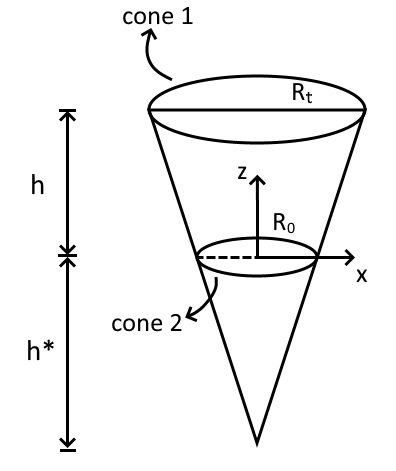
\includegraphics[clip=true,height=0.5\textwidth]{TruncatedConeAnswer01.png}\\\end{center}In the same way to determine the mass of the fluid in the container of problem 6a and as the density of the fluid is constant, the mass is given by:\\\(m=\rho \int d v\)\\\\\(m=\rho\left\{\frac{1}{3} \pi R_{0}{ }^{2} h+\frac{1}{3} \pi h R_{t} R_{0}+\frac{1}{3} \pi h R_{t}^{2}\right\}\)\\\\Solution:\\\(V=\frac{1}{3} \pi R_{t}^{2}\left\{h+\frac{h R_{0}}{R_{t}-R_{0}}\right\}-\frac{1}{3} \pi R_{0}^{2}\left\{\frac{h}{R t-R_{i}}\right\} \\ m=\rho\left\{\frac{1}{3} \pi R_{0}{ }^{2} h+\frac{1}{3} \pi h R_{t} R_{0}+\frac{1}{3} \pi h R_{t}^{2}\right\}\)\ETrule\subsection{Varying Density in a Truncated Cone}
If the density of the fluid varies linearly according to : \\\(\rho(z)=\rho_{0}-a z\)\\\\The weight of the fluid is given as: \\\(\begin{aligned}W &=\int_{0}^{h}\left(\rho_{0}-a z\right) g \pi\left\{\frac{R_{t}-R_{0}}{h} z+R_{0}\right\}^{2} d z \\&=\rho_{0} g \pi \int_{0}^{h}\left\{\left(\frac{R_{t}-R_{0}}{h}\right)^{2} z^{2}+2 \frac{R_{0}}{h}\left(R_{t}-R_{0}\right) z+R_{0}^{2}\right\} d z\\&-a g \pi \int_{0}^{h}\left\{\left(\frac{R_{t}-R_{0}}{h}\right)^{2} z^{3}+2 \frac{R_{0}}{h}\left(R_{t}-R_{0}\right) z^{2}+R_{0}^{2} z\right\} d z\\&=\rho_{0} g \pi\left\{\left(\frac{R_{t}-R_{0}}{h}\right)^{2} \frac{1}{3} z^{3}+\frac{R_{0}}{h}\left(R_{t}-R_{0}\right) z^{2}+\left.R_{0}^{2} z\right|_{0} ^{h}\right\}\&-a g \pi\left\{\frac{1}{4}\left(\frac{R_{t}-R_{0}}{h}\right)^{2} z^{4}+\frac{2}{3} \frac{R_{0}}{h}\left(R_{t}-R_{0}\right) z^{3}+\left.\frac{R_{0}^{2}}{2} z^{2}\right|_{0} ^{h}\right\}\&W=\rho_{0} g \pi h\left\{\frac{1}{3} R_{t}^{2}+\frac{1}{3} R_{t} R_{0}+\frac{1}{3} R_{0}^{2}\right\}-a g \pi h^{2}\left\{\frac{1}{4} R_{t}^{2}+\frac{1}{6} R_{t} R_{0}+\frac{1}{12} R_{0}^{2}\right\}\end{aligned}\)\\\\Solution:\\\(W=\frac{1}{3} \rho_{0} g \pi h\left\{\left(R_{t}+R_{0}\right)^{2}-R_{t} R_{0}\right\}-\frac{1}{4} \operatorname{ag\pi h}^{2}\left\{\left(R_{t}+R_{0}\right)^{2}-\frac{2}{3}\left(R_{t} R_{0}+R_{0}^{2}\right)\right\}\)\ETrule\end{document}